Determining the high-level control-flow structure from a RTL description
of a circuit would be difficult both automatically and manually.
Extracting from a high level input source manually is easier but it would
be challenging for larger designs, however it can be easily automated by
transforming the input into a control and data flow graph (CDFG).
StitchUp can automatically perform this extraction as a compiler flag
for the LegUp HLS tool.

\begin{figure}[t]
\centering
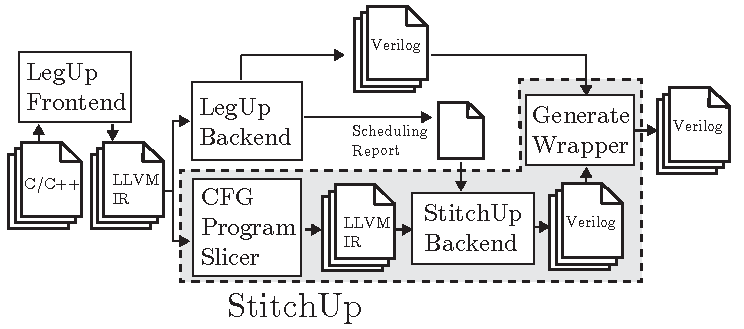
\includegraphics[width=3.5in]{./imgs/tool-flow.pdf}
\caption{Tool Flow Overview diagram}
\label{fig:tool_flow_diagram}
\end{figure}

LegUp is an open source HLS tool built upon LLVM intermediate representation (LLVM-IR) which has
a similar level of abstraction to assembly code.
LLVM-IR has two important features for writing compiler optimisations:
firstly all instructions are in single static assignment form (SSA) where every variable is only
assigned once; and secondly instructions are grouped into straight-line sequences known as basic blocks (BB)
where there is only one entry branch at the very start of the block, and one exit branch at the very end.

Figure \ref{fig:tool_flow_diagram} shows the transformation of an input C program
to a Control-flow protected
Verilog circuit description, with StitchUp sections highlighted in grey.
Initially the C input is passed into the LegUp frontend which is
a series of LLVM passes that
perform various tasks such as annotating instructions with pipelining information.
This outputs an LLVM-IR represnetation which is passed both into the backend of LegUp,
to generate the
original unprotected circuit, and into the frontend of StitchUp to generate a circuit
consisting of just the control-flow structure.
Finally a wrapper script connects the original circuit to the duplicate control-flow circuit
along with comparison logic to ensure that the state registers match.

\begin{figure}[t]
\centering
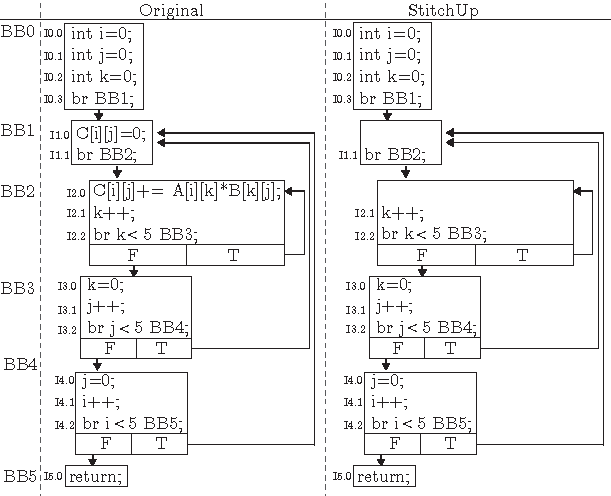
\includegraphics[width=3.5in]{./imgs/mmm_cdfg_v2.pdf}
\caption{Control-Data-Flow Diagram for Matrix Multiplication example}
\label{fig:mmm_cdfg}
\end{figure}

\subsection{Extracting the Control Instruction Set}
The LLVM-IR which is passed into the frontend of StitchUp is naturally arranged into a Control and Dataflow graph (CDFG) format,
where each node of the graph is a basic block and edges are the branches between them.
An example of the CDFG for the matrix multiplication in listing \ref{lst:MMM}
is shown on the left side of Figure \ref{fig:mmm_cdfg}.

The aim of the StitchUp frontend is to extract all SSA instructions that influence any branch decision and collect them into what
we refer to as a Control Structure Instruction Set (CSIS), which can then be used to generate a control structure only circuit.
In Figure \ref{fig:mmm_cdfg} the original CDFG and StitchUp CDFG can be seen side by side, the CSIS for this example
is every instruction within the StitchUp CDFG and it can be seen that the floating point inner dot product calculation
is not there since it has no impact on any control decision.

In order to automatically extract the $CSIS$ a backwards analysis walks up from the final node of the CDFG to the starting node, analysing
the code as it goes and creating a $CSIS_{i}$ where $i$ is the current node.
The overall $CSIS$ for the input is $CSIS_s$ where $s$ is the starting node of the CDFG.
Constructing the $CSIS_i$ for each node $i$ requires the following three steps:
\begin{enumerate}
    \item For all successor nodes, $j$, of $i$ add every element of $CSIS_j$ to $CSIS_i$.
    \item All branch instructions and operands are added to $CSIS_i$
    \item Any instruction within $i$ that is used as an operand by an element of $CSIS_i$ is added to $CSIS_i$
\end{enumerate}

\begin{algorithm}[t]
\caption{CSIS Extraction Static Analysis Algorithm
\label{alg:CSIS-extraction}}
    \begin{algorithmic}
        \INPUT a program, $P$, which is a set of Basic Blocks, \{$BB_0$, ..., $BB_N$\}
        \OUTPUT $P'$ a program containing only the instructions $I_c$ that are part of the control structure.
        \Statex
        \While{$C_{CSIS}$ != $P_{CSIS}$}
            \State $P_{CSIS} \gets \{CSIS_{BB0}, \dots,  CSIS_{BBN}$\}
            \For{\textbf{each} $B \in \{BB_{N},\dots,BB_{0}\}$}
                \\\hrulefill
                \For{\textbf{each} $S \in Successor(B)$}\Comment{Rule 1}
                    \For{\textbf{each} $I_{c} \in CSIS_{S}$}
                        \State $CSIS_B \cup \{I_{c}\}$
                    \EndFor
                \EndFor
                \\\hrulefill

                \State $T = TerminatingInstruction(B)$\Comment{Rule 2}
                \State $CSIS_{B} \cup \{T\}$
                \For{\textbf{each} $op \in T$}
                    \State $CSIS_{B} \cup \{op\}$
                \EndFor
                \\\hrulefill

                \For{\textbf{each} $I \in reverse(B)$}\Comment{Rule 3}
                    \For{\textbf{each} $I_c \in CSIS_{B}$}
                        \For{\textbf{each} $op_c \in I_c$}
                            \If{$I == op_{c}$}
                                \State $CSIS_{B} \cup \{I\}$
                            \EndIf
                        \EndFor
                    \EndFor
                \EndFor
            \EndFor
        \EndWhile
    \end{algorithmic}
\end{algorithm}

Applying the anaysis to the matrix multiplication example in Figure \ref{fig:mmm_cdfg} the
following steps are required to extract the control-flow structure:

\vspace{1mm}
\noindent
\textbf{Initially} $CSIS_{i} = \emptyset$ for all basic blocks $i$

\vspace{1pt}
\noindent
\hrulefill

\vspace{1mm}
\noindent
\textbf{Iteration 1:}

\vspace{-2pt}
$CSIS_{BB4}$: add I5.0:\emph{return} using rule 1

\vspace{-2pt}
$CSIS_{BB4}$ = \{I5.0:\emph{return}\}

\vspace{1mm}
\noindent

The analysis will continue in this fashion looping over all the Basic Blocks until a fixed
point on every $CSIS$ is obtained.
Once this has been completed it then uses the topmost $CSIS$, in this case $CSIS_{BB0}$ to
generate an LLVM-IR program containing only the control structure of the original
source.

The output of the StitchUp frontend along with the scheduling report from LegUp
implementation of the original circuit are passed into the StitchUp backend, which identical
to the LegUp Backend with a few modifications to the FSM generation.
LegUp schedules operations in such a way that if an instruction requires more than a single
clock cycles to execute then an FSM state is created for each clock cycle.
This means that if instructions are removed via the StitchUp analysis then potentially
the FSM for the StitchUp circuit could be generated missing these extra scheduling states.
For this reason the scheduling report is used to detect instances of where this situation has occurred,
and include these lost states into the StitchUp FSM.


Finally the wrapper scripts take the original LegUp circuit and the StitchUp circuit and
connect them together.
To do this the scripts expose the FSM state registers for each of the circuits and
generate logic to inspect them every clock cycle.
AXI interfaces are also generated, so that the circuits can be easily tested on Xilinx Zynq devices.
